\documentclass[a4paper,12pt,twoside, openany]{book}

\usepackage[a4paper,left=1.25in,right=1in,top=0.75in, bottom=0.75in]{geometry}
\usepackage{color}
\usepackage{courier}

\usepackage{caption}
\captionsetup{labelfont=bf}
\usepackage{subcaption} 

\usepackage{tgpagella} % text only
\usepackage{mathpazo}  % math & text

\usepackage{enumitem}

\usepackage{array}
\newcolumntype{P}[1]{>{\centering\arraybackslash}p{#1}}
\newcolumntype{M}[1]{>{\centering\arraybackslash}m{#1}}

\usepackage{hyperref}
\hypersetup{
    colorlinks = true,
    linkcolor=blue,
    %anchorcolor [black]
    %citecolor [green]
    %filecolor [cyan]
    %menucolor [red]
    %runcolor [cyan - same as file color]
    %urlcolor [magenta]
    allcolors = blue
}

%\usepackage{indentfirst}
\setlength{\parindent}{0cm}
\setlength{\parskip}{6pt}

\usepackage{setspace}
\singlespacing
\usepackage{float}
\usepackage{graphicx}
\setlength{\intextsep}{-10pt}
\usepackage{mathtools}
\numberwithin{equation}{section}

\usepackage[english]{babel}
\addto{\captionsenglish}{%
  \renewcommand{\bibname}{References}
}
\usepackage{chngcntr}
\counterwithin{figure}{chapter}
\counterwithin{table}{chapter}

\setcounter{tocdepth}{1}

\usepackage{multicol}
\usepackage{multirow}
\usepackage[table,xcdraw]{xcolor}
\usepackage{longtable}

\usepackage[belowskip=-10pt,aboveskip=-15pt]{caption}
\newcommand{\squeezeup}{\vspace{-2.5mm}}
 
\usepackage{sectsty}
\chapternumberfont{\Large} 
%\chaptertitlefont{\Large}
%\sectionfont{\large}
%\subsectionfont{\normalsize}
%\subsubsectionfont{\normalsize}

\renewcommand{\thesection}{\arabic{section}}
\numberwithin{section}{chapter}

\usepackage[utf8]{inputenc}
\usepackage{fancyhdr}

\pagestyle{fancy}
\fancyhf{}
\fancyhead[LE,RO]{\footnotesize{\textit{\leftmark \\ \rightmark}}}
\fancyhead[RE,LO]{}
\fancyfoot[CE,CO]{\footnotesize{\copyright FrenusTech Pvt Ltd}}
\fancyfoot[LE,RO]{\thechapter-\thepage}

\fancypagestyle{plain}{%
\fancyhf{}
\fancyfoot[CE,CO]{\footnotesize{\copyright FrenusTech Pvt Ltd}}
\fancyfoot[LE,RO]{\thechapter-\thepage}
}

\renewcommand{\headrulewidth}{0pt}
\renewcommand{\footrulewidth}{1pt}

\begin{document}

\begin{titlepage}

\vspace{1cm}
\begin{figure}[H]
\centering

\includegraphics[totalheight=2cm]{images/frenustechLogo50-1.png}
\end{figure}
\vspace{0.5cm}

\begin{center}
\Large{\textsc{\\}}
%\vspace{0.5cm}
\hrule %hrule draws a horizontal line
\vspace{0.1in}
\begin{flushright}
\Huge{ \textbf {Zilla Interrupt Controller}}\\[0.25cm]
\normalsize{\textit{\textbf{ Architecture Version 0.9}}}\\[1cm]
\large{\textbf{Architecture Specification}}
\end{flushright}
\vspace{0.1in}
\hrule
\end{center}

\vspace{14cm}

\begin{flushright}
\textbf{Contact\\} 
\url{siddartha.hp@frenustech.com}\\
\url{consultant.rv4@frenustech.com}

\end{flushright}


\end{titlepage}

\setcounter{page}{1}
\pagenumbering{roman}

\tableofcontents
\thispagestyle{plain}
%\listoffigures

%\addcontentsline{toc}{chapter}{List of Figures}
%\thispagestyle{plain}

%\listoftables

%\addcontentsline{toc}{chapter}{List of Tables}

%\include{acronyms}

\chapter*{Preface}
\addcontentsline{toc}{chapter}{Preface}

\section*{About this specification}
\addcontentsline{toc}{section}{About this specification}



\subsection*{Intended Audience}



\section*{Using this specification}
\addcontentsline{toc}{section}{Using this specification}



\section*{Conventions}
\addcontentsline{toc}{section}{Conventions}


\section*{Feedback}
\addcontentsline{toc}{section}{Feedback}


\setcounter{page}{1}
\pagenumbering{arabic}

\chapter{Introduction}
This chapter gives an overview of the ZIC  and information about the terminology used in this document. It contains the following sections:
\begin{itemize}
    \item \hyperref[sec:about-zic-arch]{About Zilla Interrupt Controller Architecture}
    \item \hyperref[sec:terminology]{Terminology}
\end{itemize}
\newpage

\section{About Zilla Interrupt Controller architecture}
\label{sec:about-zic-arch}
The current architectural version of Zilla Interrupt Controller (ZIC) supports 48 interrupts (External, Software, and Timer). The controller can be scaled to support up to 4096 external interrupts. The role of ZIC is to determine which interrupt has to be sent to the processor core depending on the predefined level and priorities.

ZIC uses a set of memory-mapped registers and Control and Status registers (CSRs) for flow control. Memory-mapped registers are accessible via the software as well as the hardware. ZIC supports preemption of current serving interrupt based on level All the interrupts are taken in the machine privilege mode. ZIC implementation closely floors the RISC-V CLIC specifications.

The features of the Zilla interrupt controller are as follows:

\begin{enumerate}
    \item Supports up to 48 external interrupts. (Scalable up to 4096).
    \item Programmable Interrupt Levels and Priorities
    \begin{enumerate}[label=(\alph*)]
        \item Up to 8 Levels (for nesting).
        \item Up to 8 priorities in each level.
    \end{enumerate}
    \item Grouping of priority values into levels.
    \item Memory-mapped registers for control and status.
    \item Support for both direct mode and vectored mode operation.
    \item Low-Latency Interrupt Handling.
    \item An external Non-Maskable Interrupt
\end{enumerate}

\subsection{ZIC architecture specification version}

\subsection{Changes in version 1.0 of the specification}

\section{Terminology}
\label{sec:terminology}
The following sections define architectural terms used in this specification:

\subsection{Basic Terminology}

\subsection{Interrupt States}

\subsection{Interrupt Handling Modes}

\subsection{Register Access Types}


\chapter{JTAG Overview}
This chapter gives an overview of the JTAG  and partitioning of the JTAG. It contains the following sections:
\begin{itemize}
    \item \hyperref[sec:system-overview]{System Overview}
    \item \hyperref[sec:bst-arhitecture]{Boundary Scan Testing Architecture}
    \item \hyperref[sec:jtag-partitioning]{JTAG Partitioning}
\end{itemize}
\newpage

\section{System Overview}
\label{sec:system-overview}
In JTAG, testing and debugging is carried through Test Access Port (TAP) which contains four mandatory pins (TDI, TMS, TCK, TDO) and an optional pin for asynchronous reset (TRST). A  TAP/JTAG controller is a module that controls and coordinates the operations of the entire test architecture.

The Figure \ref{fig:zic_partitioning} shows the conceptual view of top level JTAG design.

\vspace{1cm}
\begin{figure}[H]
    \centering
    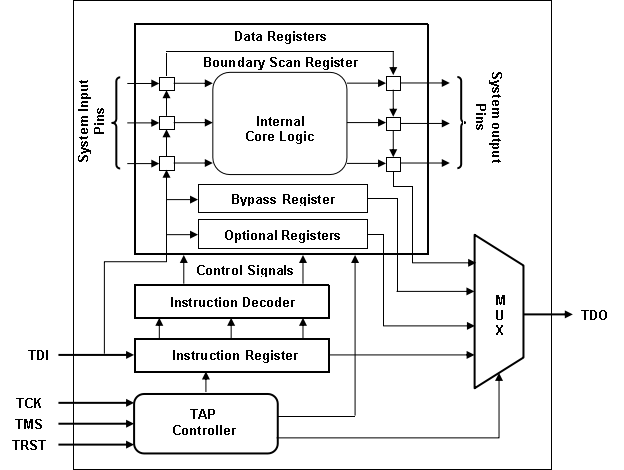
\includegraphics[width = 15cm]{images/jtag_block_diagram.png}
    \vspace{1cm}
    \caption{ZIC Partitioning}
    \label{fig:zic_partitioning}
\end{figure}
\vspace{1cm}

The sequence of operation is as follows

\begin{enumerate}
    \item The TAP controller receives TCK and interprets the signals on TMS. The TAP controller generates clock or control signals or both as required for the instruction and test data registers and for other parts of the design.
    \item  The TAP controller controls the operation (normal, shift, capture, update) while instruction decoder provides the context of the operation (i.e., to which register and associated test logic the action applies).
    \item The instruction register allows the instruction to be shifted into the design. The instruction is used to select the test to be performed or the test data register to be accessed or both.
    \item The instruction register is never undefined and always selects a single test data register to connect between TDI and TDO.
    \item The group of test data registers shall include a bypass and a boundary-scan register. It also may include any of the optional standard test data registers: the device identification, initialization data, initialization status, TMP control, and reset selection registers; and further optional design specific test data registers. 
    \item A circuit controlled by instruction decoder selects the test data register to drive the output TDO.
\end{enumerate}

\section{Boundary Scan Testing Architecture}
\label{sec:bst-arhitecture}

Boundary scan is a method for testing interconnects (wire lines) on printed circuit boards or sub-blocks inside an integrated circuit. 

\vspace{1cm}
\begin{figure}[H]
    \centering
    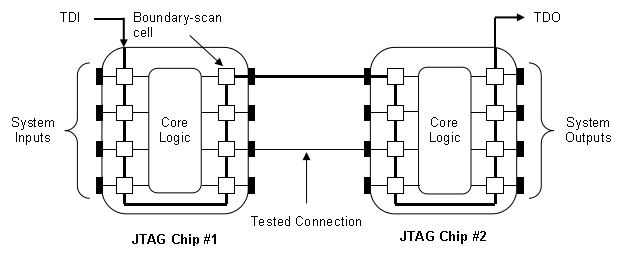
\includegraphics[width = 14cm]{images/boundary_scan_test.png}
    \vspace{1cm}
    \caption{Boundary Scan Test}
    \label{fig:bst}
\end{figure}
\vspace{1cm}

Boundary scan is also widely used for 
\begin{enumerate}
    \item Debugging - watch integrated circuit pin states
    \item Board-level test and diagnosis
    \item Test on-board interconnect among chips
    \item Test on-chip system logic
\end{enumerate}

\section{JTAG Partitioning}
\label{sec:jtag-partitioning}

 The JTAG architecture is partitioned into the following functional blocks
\begin{enumerate}
    \item \hyperref[chap:TAP]{Test Access Port (TAP)}
    \item \hyperref[chap:instruction-reg]{Instruction Register}
    \item \hyperref[chap:data-reg]{Test Data Registers}
\end{enumerate}

The instruction and test data registers shall be separate shift-register based paths that are connected in parallel and have a common serial data input and a common serial data output connected to the TAP TDI and TDO signals, respectively. 

The selection between the alternative instruction and test data register paths between TDI and TDO shall be made under the control of the TAP controller.

\chapter{Test Access Port (TAP)}
\label{chap:TAP}

This chapter gives an overview about Test Access Port (TAP) and the interface signals that control the TAP controller. It contains the following sections 

\begin{itemize}
    \item \hyperref[sec:about-tap]{About TAP}
    \item \hyperref[sec:tap-controller]{TAP Controller}
\end{itemize}
\newpage

\section{About TAP}
\label{sec:about-tap}

TAP, uses the following signals to interface and support the operation of boundary scan.
\begin{itemize}
    \item \hyperref[subsec:tck]{Test Clock}
    \item \hyperref[subsec:tms]{Test Mode Select}
    \item \hyperref[subsec:tdi]{Test Data Input}
    \item \hyperref[subsec:tdo]{Test Data Output}
    \item \hyperref[subsec:trst]{Test Reset} (optional)
\end{itemize}

Table \ref{tab:top-port} shows the top level ports and description for the same.

\vspace{1cm}
\begin{table}[H]
    \caption{Top Level port description}
    \label{tab:top-port}
    \vspace{1cm}
    \begin{tabular}{l l l p{8cm}}

    \hline
         \textbf{Port} & \textbf{Name} & \textbf{Direction} & \textbf{Description}\\ \hline \hline
        \hyperref[subsec:tck]{TCK} & Test Clock & Input & The clock input to the BST circuitry.\\  \hline
        \hyperref[subsec:tms]{TMS} & Test Mode Select & Input & Provides the control signal to determine the transitions of the TAP controller state machine.\\ \hline
        \hyperref[subsec:tdi]{TDI} & Test Data Input & Input & Serial input pin for instructions as well as test data. Data is shifted in on the rising edge of TCK. \\ \hline
        \hyperref[subsec:tdo]{TDO} & Test Data Output & Output & Serial data output pin for instructions as well as test data. Data is shifted out on the falling edge of TCK. \\ \hline
        \hyperref[subsec:trst]{TRST} & Test Reset & Input & Asynchronous active low reset to reset the TAP controller, when TRST is applied to 0.
        \\ \hline
        \end{tabular}
\end{table}
\vspace{0.5cm}

\subsection{Test Clock, TCK}
\label{subsec:tck}
The dedicated TCK input is included so that the serial test data path between components can be used independently of component-specific system clocks, which may vary significantly in frequency from one component to the next. The provision of an independent clock helps ensure that test data can be moved to or from a component without changing the state of the on-chip system logic. 

The clock input to the BST circuitry. Some operations occur at the rising edge, while others occur at the falling edge. The clock input waveform should have a 50\% duty cycle.


\subsection{Test Mode Select, TMS}
\label{subsec:tms}
The value of the signal present at TMS at the time of a rising edge at TCK determines the next state of the TAP controller, the circuit that controls test operations. The signal presented at TMS shall be sampled by the test logic on the rising edge of TCK

\subsection{Test Data Input, TDI}
\label{subsec:tdi}
Serial test instructions and test data are received by the test logic at TDI. Values presented at TDI are clocked into the selected register (instruction or test data) on a rising edge of TCK.
The data pins (TDI and TDO) provide for serial movement of test data through the circuit. When data is being shifted from TDI toward TDO, test data received at TDI shall appear without inversion at TDO after a number of rising and falling edges of TCK determined by the length of the instruction or test data register selected.

\subsection{Test Data Output, TDO}
\label{subsec:tdo}
TDO is the serial output for test instructions and data from the test logic defined in this standard. Changes in the state of the signal driven through TDO shall occur only on the falling edge of TCK, i.e the contents of the selected register (instruction or data) are shifted out of TDO on the falling edge of TCK.

To help ensure a race-free operation, changes on TAP inputs (TMS and TDI) are clocked into the test logic defined by this standard on the rising edge of TCK while changes at the TAP output (TDO) occur on the falling edge of TCK. Similarly, for test logic able to drive or receive signals from system pins (e.g., the boundary-scan register), signals driven out of the component from the test logic change state on the falling edge of TCK, while those entering the test logic are clocked in on the rising edge. 

\subsection{Test Reset, TRST}
\label{subsec:trst}
The optional TRST input provides for asynchronous initialization, principally at power-up, of the TAP controller. TRST is required when the test logic does not power-up in a known and controlled state. If TRST is included in the TAP, the TAP controller shall be asynchronously reset to the Test-Logic-Reset state, when a logic 0 is applied to TRST. To avoid race conditions in the test logic, TMS should be held at 1 while the signal applied at TRST changes from 0 to 1.

\newpage

\section{TAP Controller}
\label{sec:tap-controller}

The IEEE Std. 1149.1 test access port (TAP) controller, a 16-state state machine clocked on the rising edge of TCK. 

TAP controller is a synchronous finite state machine that responds to changes at the TMS and TCK signals of the TAP, controls the behavior of the test logic, and maintains synchronization across all components on a test scan chain to permit shifting, capturing, and updating of data in the device.

\vspace{1cm}
\begin{figure}[H]
    \centering
    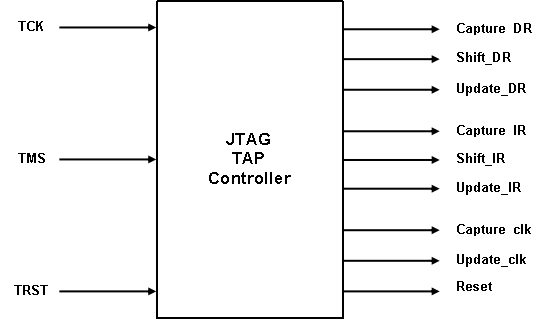
\includegraphics[width = 10cm]{images/jtag_tap_controller.png}
    \vspace{1cm}
    \caption{TAP Controller}
    \label{fig:tap-controller}
\end{figure}

\subsection{TAP Controller Ports}
\label{subsec:tap-controller-ports}

\begin{longtable}{l l p{9.5cm}}
    \caption{TAP controller port description}
    \label{tab:tap-ports}\\
    \hline
         \textbf{Port Name} & \textbf{Direction} & \textbf{Description}\\ \hline \hline
         \hyperref[subsec:tck]{TCK} & Input & Test Clock Input \\ \hline
         \hyperref[subsec:tms]{TMS} & Input & Test Mode Select Input \\ \hline
         \hyperref[subsec:trst]{TRST} & Input & Test Reset Input \\ \hline
         \hyperref[subsubsec:capture-dr]{Capture\_DR} & Output & This flag is set when the controller is in Capture\_DR State. It Controls the Capture operation in the Data Register Scan Path. \\ \hline
         \hyperref[subsubsec:shift-dr]{Shift\_DR} & Output & This flag is set when the controller is in Shift\_DR State. It controls the Shift operation in Data Register Scan Path. \\ \hline
         \hyperref[subsubsec:update-dr]{Update\_DR} & Output & This flag is set when the controller is in Update\_DR State. It controls the Update operation in the Data Register Scan Path. \\ \hline
         \hyperref[subsubsec:capture-ir]{Capture\_IR} & Output & This flag is set when the controller is in Capture\_IR State. It controls the Capture operation in the Instruction Register Scan Path. \\ \hline
         \hyperref[subsubsec:shift-ir]{Shift\_IR} & Output & This flag is set when the controller is in Shift\_IR State. It controls the Shift operation in the Instruction Register Scan Path. \\ \hline
         \hyperref[subsubsec:update-ir]{Update\_IR} & Output & This flag is set when the controller is in Update\_IR State. It controls the Update operation in the Instruction Register Scan Path. \\ \hline
         Capture\_clk & Output & It is the posedge of the TCK clock. This clock is used for Capture and Shift Operations. \\ \hline
         Update\_clk & Output & It is the negedge of the TCK clock. This clock is used for Update Operations. \\ \hline
         Reset & Output & This signal is set when the state is in \texttt{TEST\_LOGIC\_RESET} State.\\ \hline
\end{longtable}

\section{TAP Controller FSM}
\label{subsec:tap-fsm}

All state transitions of the TAP controller shall occur based on the value of TMS at the time of a rising edge of TCK. The transitions are as shown in Figure \ref{fig:tap-controller-fsm}.

\vspace{1cm}
\begin{figure}[H]
    \centering
    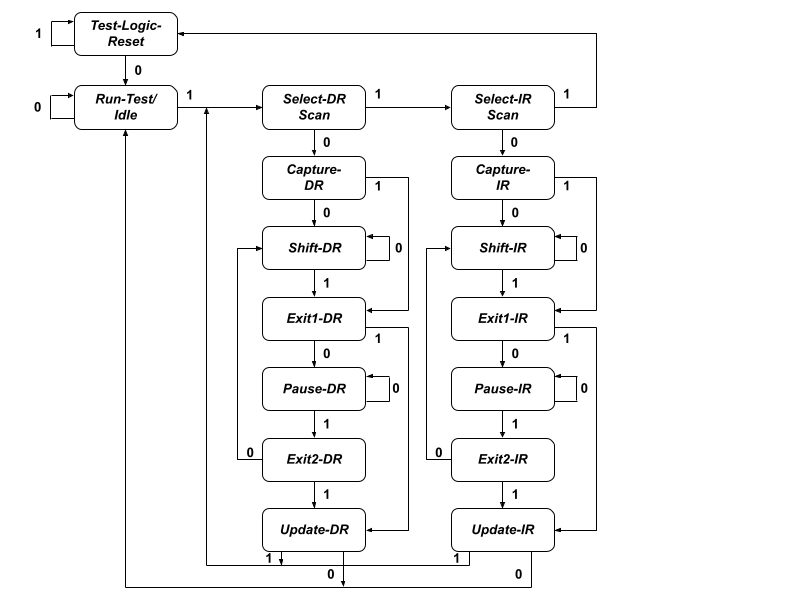
\includegraphics[width = 18cm]{images/tap_state_diagram.png}
    \vspace{1cm}
    \caption{TAP Controller FSM}
    \label{fig:tap-controller-fsm}
\end{figure}

\newpage

\subsection{TAP Controller Initialization}
\label{subsec:tap-controller-initial}

The TAP controller shall be forced into the Test-Logic-Reset controller state at power-up either by use of the TRST signal or as a result of circuitry built into the test logic or both.

The TAP controller shall not be initialized by operation of any system input, such as a system reset.

Where a dedicated reset pin (TRST) is provided to allow initialization of the TAP controller, initialization shall occur asynchronously (without dependence on TCK or any other clock) when the TRST input changes to the low logic level.

Where the TAP controller is initialized at power-up by operation of circuitry built into the test logic, the result shall be equivalent to that which would be achieved by application of a logic 0 to a TRST input.

\subsubsection{Test-Logic-Reset}
\label{subsubsec:test-logic-reset}
It resets the JTAG circuits. Whenever the TRST (optional) signal is asserted, it goes back to this state. The TAP controller state machine is designed so that, no matter what the initial state of the controller is, the Test-Logic-Reset state can be entered by holding TMS at high and pulsing TCK five times. Thus if we don’t have the TRST signal then we can still reset the circuit.

\subsubsection{Run-Test/Idle}
\label{subsubsec:run-test-idle}
In this state, the test logic in the IC is active only if certain instructions are present. For example, if an instruction activates the self test, then it is executed when the controller enters this state. The test logic in the IC is idle otherwise. The instruction does not change while the TAP controller is in this state.

\subsection{Select-IR Scan}
\label{subsec:select-ir}
This state controls whether or not to enter the Instruction Path. The Controller can return to the Test-Logic-Reset state otherwise. If TMS is held low and a rising edge is applied to TCK when the controller is in this state, then the controller moves into the Capture-IR state and a scan sequence for the instruction register is initiated. If TMS is held high and a rising edge is applied to TCK, the controller returns to the Test-Logic-Reset state.

\subsubsection{Capture-IR}
\label{subsubsec:capture-ir}
This is a temporary state in which a pattern of fixed logic values is parallel-loaded into specific bits of the instruction register shift-capture path on the rising edge of TCK. When the TAP controller is in this state and a rising edge is applied to TCK, the controller enters either the Exit1-IR state if TMS is held at 1 or the Shift-IR state if TMS is held at 0.

\subsubsection{Shift-IR}
\label{subsubsec:shift-ir}
In this state, the instruction register gets connected between TDI and TDO, and the captured pattern gets shifted on each rising edge of TCK from TDI to TDO. The instruction available on the TDI pin is also shifted into the instruction register. When the TAP controller is in this state and a rising edge is applied to TCK, the controller either enters the Exit1-IR state if TMS is held at 1 or remains in the Shift-IR state if TMS is held at 0.

\subsubsection{Exit1-IR}
\label{subsubsec:exit1-ir}
This state controls whether to enter the Pause-IR state if TMS holds low or Update-IR state if TMS holds high at the rising edge of TCK.

\subsubsection{Pause-IR}
\label{subsubsec:pause-ir}
This state allows shifting of the instruction register to be halted temporarily. The controller remains in this state while TMS is low. When TMS is set and a rising edge is applied to TCK, the controller moves on to the Exit2-IR state.

\subsubsection{Exit2-IR}
\label{subsubsec:exit2-ir}
If TMS is held high and a rising edge is applied to TCK while in this state, termination of the scanning process results, and the TAP controller enters the Update-IR controller state. If TMS is held low and a rising edge is applied to TCK, the controller enters the Shift-IR state.

\subsubsection{Update-IR}
\label{subsubsec:update-ir}
In this state, the bits in the instruction register shift-capture path are latched onto the parallel output on the falling edge of TCK. Once the new value has been latched, it becomes the current instruction. When the TAP controller is in this state and a rising edge is applied to TCK, the controller enters the Select-DR Scan state if TMS is held at 1 or the Run-Test/Idle state if TMS is held at 0.

\subsection{Select-DR Scan}
\label{subsec:select-dr}
This state controls whether to enter the Data Path or the Select-IR-Scan state. If TMS is held low and a rising edge is applied to TCK when the controller is in this state, the controller moves into the Capture-DR state and a scan sequence for the selected test data register is initiated. If TMS is held high and a rising edge is applied to TCK, the controller moves on to the Select-IR-Scan state.

\subsubsection{Capture-DR}
\label{subsubsec:capture-dr}
In this state, the data is parallel-loaded into the data registers selected by the current instruction on the rising edge of TCK. When the TAP controller is in this state and a rising edge is applied to TCK, the controller enters either the Exit1- DR state if TMS is held at 1 or the Shift-DR state if TMS is held at 0.

\subsubsection{Shift-DR}
\label{subsubsec:shift-dr}
This state is analogous to \hyperref[subsubsec:shift-ir]{Shift-IR} in the Instruction Path.

\subsubsection{Exit1-DR}
\label{subsubsec:exit1-dr}
This state is analogous to \hyperref[subsubsec:exit1-ir]{Exit1-IR} in the Instruction Path.

\subsubsection{Pause-DR}
\label{subsubsec:pause-dr}
This state is analogous to \hyperref[subsubsec:pause-ir]{Pause-IR} in the Instruction Path.

\subsubsection{Exit2-DR}
\label{subsubsec:exit2-dr}
This state is analogous to \hyperref[subsubsec:exit2-ir]{Exit2-IR} in the Instruction Path.

\subsubsection{Update-DR}
\label{subsubsec:update-dr}
This state is analogous to \hyperref[subsubsec:update-ir]{Update-IR} in the Instruction Path.

\chapter{Instruction Register}
\label{chap:instruction-reg}
This chapter gives an overview of the design and operation of Instruction Register. It contains the following sections:
\begin{itemize}
    \item \hyperref[sec:about-instruction-reg]{About Instruction Register}
    \item \hyperref[sec:design-instruction-reg]{Design of Instruction Register}
    \item \hyperref[sec:operation-instruction-reg]{Operational Overview}
    \item \hyperref[sec:instruction-decoder]{Instruction Decoder}
\end{itemize}

\newpage

\section{About Instruction Register}
\label{sec:about-instruction-reg}
The instruction register allows an instruction to be shifted into the design. The instruction is used to select the test to be performed or the test data register to be accessed or both. Also, store JTAG instructions for instruction decoder.

\section{Design of Instruction Register}
\label{sec:design-instruction-reg}
The purpose of Instruction Register is to shift in instruction through TDI and having the provision to store the instruction till a new instruction is fully shifted in. Typically an IR has two registers inside it as shown below. The Hold Register stores the previous instruction and the Shift Register is used to shift-in the next instruction without affecting the previous instruction’s execution. 

\vspace{1cm}
\begin{figure}[H]
    \centering
    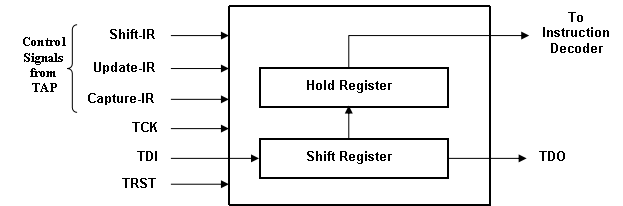
\includegraphics[width = 12cm]{images/instruction_register_top.png}
    \vspace{1cm}
    \caption{Top Level View of Instruction Register}
    \label{fig:instruction-reg-top}
\end{figure}
\vspace{1cm}

The instruction shifted into the instruction register shall be latched such that \linebreak changes in the effect of an instruction occur only in the Update-IR and Test-Logic-Reset TAP controller states.

\vspace{1cm}
\begin{figure}[H]
    \centering
    
\includegraphics[width = 10cm]{images/jtag_instruction_register.png}
    \vspace{1cm}
    \caption{JTAG Instruction Register}
    \label{fig:jtag-instruction-reg}
\end{figure}
\vspace{1cm}

The control signals to the Instruction register originates from the TAP controller and depending upon the FSM state can either cause a shift-in/shift-out through the Shift Register (serial update operation in Shift-IR state ), or cause the contents of the Shift Register to be passed across to the Hold Register (parallel update operation in Update-IR state). 

\subsection{Instruction Register Ports}

\begin{longtable}{l l p{9.5cm}}
    \caption{Instruction Register port description}
    \label{tab:instruction-reg-ports}\\
    \hline
         \textbf{Port Name} & \textbf{Direction} & \textbf{Description}\\ \hline \hline
        \hyperref[subsec:trst]{TRST} & Input & Asynchronous Active low reset: If asserted default IDCODE Instruction is selected. \\ \hline
        \hyperref[subsec:tdi]{TDI} & Input & Test Data Input \\ \hline
        Reset & Input & Asserted when the state is in the TEST\_LOGIC\_RESET state. During the posedge of Update\_clk if asserted default IDCODE instruction is selected. \\ \hline
        Capture\_clk & Input & Capture\_clk (posedge of TCK) captures the instruction. \\ \hline
        Capture\_IR & Input & Controls the Capture Operations, captures the instruction during Capture\_IR stage in the posedge of Capture\_clk if no TRST and Reset is there. Basically it captures 4’b0001 instructions when Capture\_IR is asserted. The JTAG standard requires the last two bits ‘01’. \\ \hline
        Shift\_IR & Input & Controls the Shift Operation, Shifts the TDI bit during the posedge of Capture\_clk from one cell to other cell. \\ \hline
        Update\_clk & Input & Update\_clk (negedge of TCK) updates the instruction. \\ \hline
        Update\_IR & Input & Controls the Update\_IR Operations, during the posedge of Update\_clk if no TRST and Reset then Shift Stage instructions are updated to instr\_reg\_out. \\ \hline
        instr\_reg\_out & Output & Instruction register output gets the instruction to be performed by JTAG. \\ \hline
        ir\_shift\_out & Output & 1-bit instruction bit shifted out during Shift\_IR operation Stage. \\ \hline
        bypass\_sel & Output & BYPASS Instruction is executed, if
        
        \texttt{instr\_reg\_out = 4’hF}. \\ \hline
        idcode\_sel & Output & IDCODE Instruction is executed, If
        
        \texttt{instr\_reg\_out = 4’h2}. \\ \hline
        usercode\_sel & Output & USER\_CODE Instruction is executed, if
        
        \texttt{instr\_reg\_out = 4’h6}. \\ \hline
        userdata\_sel & Output & USER\_DATA Instruction is executed, if
        
        \texttt{instr\_reg\_out = 4’h8}. \\ \hline
\end{longtable}

\newpage

\section{Operational Overview}
\label{sec:operation-instruction-reg}
All operations of shift-register stages shall occur on the rising edge of TCK after entry into a controller state.

\begin{enumerate}
    \item The clock input (Clock-IR) to the register in the serial path is applied only during the Capture-IR and Shift-IR TAP controller states.
    \item The data present at the parallel output of the instruction register shall be latched from the shift-register stage on the falling edge of TCK in the Update-IR controller state. The clock input (Update-IR) to the hold register is applied only during the Update-IR TAP controller state.
    \item The parallel output (labeled Instruction bit) is updated at the end of the \linebreak instruction-scan cycle during the Update-IR controller state.
    \item The parallel output is reset in the Test-Logic-Reset controller state as a result of a logic 0 received at the Reset input of the cell. After entry into the Test-Logic-Reset controller state as a result of the clocked operation of the TAP controller, the IDCODE instruction (or, if there is no device identification register, the BYPASS instruction) shall be latched onto the instruction register output on the falling edge of TCK.
    \item If the TRST input is provided and a low signal is applied to the input, the latched instruction shall change asynchronously to IDCODE (or, if no device identification register is provided, to BYPASS).
    \item JTAG standard requires the last two bits of parallel load = ‘01’ which is closest to TDO and Scan operation does not interfere with instruction decoder.
\end{enumerate}

\vspace{0.5cm}
\begin{figure}[H]
    \centering
    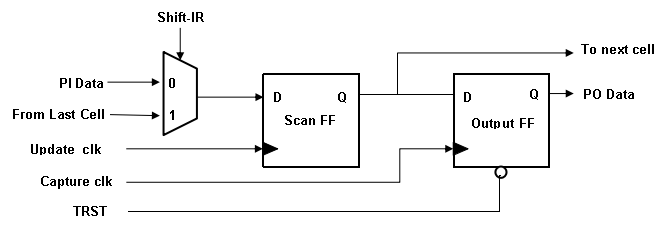
\includegraphics[width = 15cm]{images/instruction_register_cell.png}
    \vspace{1cm}
    \caption{Instruction Register Cell}
    \label{fig:instruction-reg-cell}
\end{figure}

\newpage

\section{Instruction Decoder}
\label{sec:instruction-decoder}
The instruction from the Instruction Register (IR) is fed to a decoder logic, which selects the Data Register for JTAG operation. We assign a unique value (or opcode) to each and every Data Register in the JTAG. In order to select a Data Register, we load the IR with the corresponding opcode and the Instruction Decoder decodes the value and establishes an access path between the TDI/TDO and the required Data Register.

\vspace{1cm}
\begin{figure}[H]
    \centering
    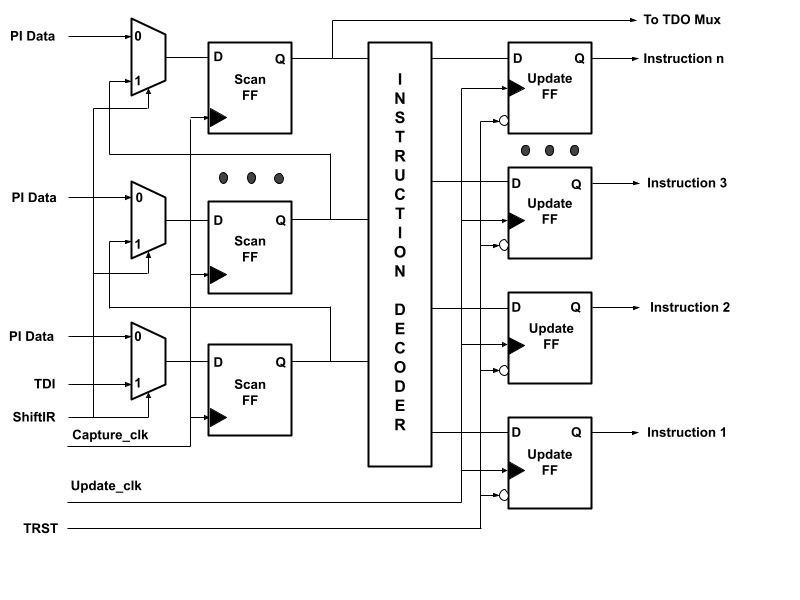
\includegraphics[width = 15cm]{images/instruction_register_shift_update.png}
    \vspace{1cm}
    \caption{Instruction decoder between shift and update stages}
    \label{fig:instruction-decoder}
\end{figure}
\vspace{1cm}

The advantage is that the instruction decodes are now updated by a clock and are therefore glitch-free. The number of update flops or latches is now the same as the number of instructions, not the number of instruction register bits. Note that “Instruction 1” is set “on” by the “Reset” signal; this would be the mandatory BYPASS or IDCODE instruction decode.


\chapter{Test Data Registers}
\label{chap:data-reg}

This chapter gives an overview of data registers and their operation. It contains the following sections:
\begin{itemize}
    \item \hyperref[sec:about-data-regs]{About Data Registers}
    \item \hyperref[sec:data-regs-types]{Types of Data Registers}
\end{itemize}

\newpage

\section{About Data Registers}
\label{sec:about-data-regs}

The test logic architecture contains two test data registers (TDRs); the bypass and boundary-scan registers. In addition, the designs of other standard optional test data registers are defined: the device identification, electronic chip identification, initialization data, initialization status, TMP status, and reset selection registers.

The bypass, boundary-scan, and optional test data registers are realized as a set of shift-register based elements connected in parallel between a common serial input and a common serial output. Selection of the register that forms the serial path at a given time is controlled from the instruction register.

\vspace{1.25cm}
\begin{figure}[H]
    \centering
    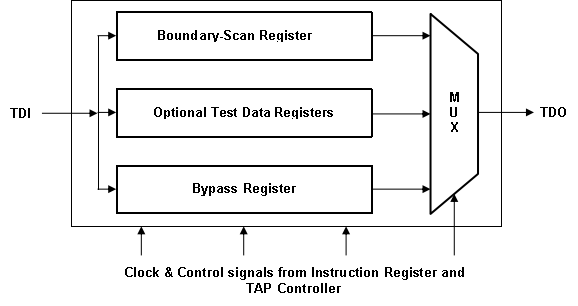
\includegraphics[width = 15cm]{images/test_data_registers.png}
    \vspace{1cm}
    \caption{JTAG Test data Registers Overview}
    \label{fig:data-regs-overview}
\end{figure}
\vspace{1cm}

Bypass Register provides a single-bit, which is the minimum length for any TDR serial connection through the circuit when none of the other test data registers is selected. This register can, for example, be used to allow test data to flow through a particular component to other components in a product without affecting the normal operation of the particular component.

Boundary-Scan Register allows testing of board interconnections, detecting typical production defects such as opens, shorts, and so on. It also allows access to the inputs and outputs of components when testing their system logic or sampling of signals flowing through the system inputs and outputs.

Boundary-scan register is not in the scope of current implementation. Only BYPASS, IDCODE, USERCODE, and USERDATA registers are implemented as a part of JTAG.

\section{Design of JTAG Register}

\vspace{1cm}
\begin{figure}[H]
    \centering
    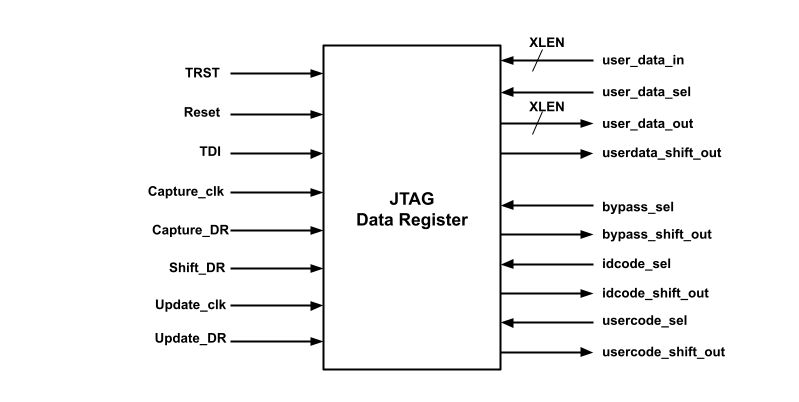
\includegraphics[width = 15cm]{images/jtag_data_register.png}
    \vspace{1cm}
    \caption{JTAG Test data Register}
    \label{fig:data-reg}
\end{figure}
\vspace{1cm}

\subsection{Data Register Ports}

\begin{longtable}{l l p{9.5cm}}
    \caption{Data Register port description}
    \label{tab:data-reg-ports}\\
    \hline
         \textbf{Port Name} & \textbf{Direction} & \textbf{Description}\\ \hline \hline
        \hyperref[subsec:trst]{TRST} & Input & Asynchronous Active low reset: If asserted default IDCODE Instruction is selected. \\ \hline
        Reset & Input & This signal is asserted when the state is in \texttt{TEST\_LOGIC\_RESET} State. \\ \hline
        \hyperref[subsec:tdi]{TDI} & Input & Test Data Input \\ \hline 
        Capture\_clk & Input & Capture\_clk (posedge of TCK) captures the data \\ \hline
        Capture\_DR & Input & Controls the Capture Operation of Data Register. Captures the data in the posedge of Capture\_clk if no TRST and Reset is there. \\ \hline
        Shift\_DR & Input & Controls the Shift Operation of Data Register. Shift the data bits from one register to another register in the posedge of Capture\_clk. \\ \hline
        Update\_clk & Input & Update\_clk (negedge of TCK) updates the data.\\ \hline
        Update\_DR & Input & Controls the Update Operation of Data Register. Update the data bits in the posedge of Update\_clk if no TRST. \\ \hline
        user\_data\_in & Input & XLEN bits of User Data Input coming from the top module specified by the user. \\ \hline
        user\_data\_sel & Input & Selects the USER DATA Register. \\ \hline
        user\_data\_out & Output & User Data Output Signal updates in the Update\_DR State. \\ \hline
        userdata\_shift\_out & Output & User Data Shift out bit shifted data bit in the Shift\_DR State.  \\ \hline
        bypass\_sel & Input & Selects the Bypass Register  \\ \hline
        bypass\_shift\_out & Output & Bypass shift bit in the Shift\_DR state.  \\ \hline
        idcode\_sel & Input & Selects the IDCODE Register. \\ \hline
        idcode\_shift\_out & Output & Idcode shift bit in the Shift\_DR State  \\ \hline
        usercode\_sel & Input & Selects the USER CODE Register.  \\ \hline
        usercode\_shift\_out & Output & User code shift bit in the Shift\_DR State.  \\ \hline
\end{longtable}

\section{Types of Data Registers}
\label{sec:data-regs-types}

The different types of Data Register are as follows:
\begin{enumerate}
    \item \hyperref[subsec:bypass-reg]{BYPASS register}
    \item \hyperref[subsec:idcode-reg]{IDCODE register}
    \item \hyperref[subsec:device-id-reg]{Device Identification register}
    \item \hyperref[subsec:userdata-reg]{USERDATA Register}
\end{enumerate}

\subsection{BYPASS register}
\label{subsec:bypass-reg}
The BYPASS mode is activated when an instruction code of all 1’s is loaded in the instruction register. In this register the scan data passes through a device once the TAP controller is in the SHIFT\_DR state. In this state, data signals are clocked into the bypass register from TDI on the rising edge of TCK and out of TDO on the falling edge of the same clock pulse.

\subsection{IDCODE register}
\label{subsec:idcode-reg}
The IDCODE instruction mode is used to identify the devices in an IEEE Std. 1149.1 chain. When IDCODE is selected, the device identification register is loaded with the 32-bit vendor-defined identification code (\texttt{32'h1495\_11c3}). The device ID register is connected between the TDI and TDO ports, and the device IDCODE is shifted out.

\subsection{Device Identification register}
\label{subsec:device-id-reg}
The USERCODE instruction mode is used to examine the user electronic signature (UES) within the devices along an IEEE Std. 1149.1 chain. When this instruction is selected, the device identification register is connected between the TDI and TDO ports. The user-defined UES is shifted into the device ID register in parallel from the 32-bit USERCODE register. The UES is then shifted out through the device ID register. The UES value is not user defined until after the device has been configured. Before configuration, the UES value is set to the default value.

\subsection{USERDATA Register}
\label{subsec:userdata-reg}
In this register 8 bit user data input value is captured in the Capture\_DR Stage and then shifted in the Shift\_DR Stage in the posedge of Capture\_clk if no TRST and Reset is there. The shifted bits are updated to user data output in the Update\_DR Stage in the posedge of Update\_clk.


\chapter{Test Data Out Multiplexer (TDO MUX)}
\label{chap:tdo-mux}

This chapter gives an overview of TDO MUX and their operation. It contains the following sections:
\begin{itemize}
    \item \hyperref[sec:about-tdo-mux]{About TDO MUX}
\end{itemize}

\newpage

\section{About TDO MUX}
\label{sec:about-tdo-mux}
Based on the instruction selected by instruction decoder, The TDO MUX Block multiplexes the shifted bit from instruction register and data register to TDO in the negedge of TCK if no TRST is there else TDO gets 1’b0 value.

\vspace{1cm}
\begin{figure}[H]
    \centering
    
\includegraphics[width = 10cm]{images/jtag_tdo_mux.png}
    \vspace{1cm}
    \caption{JTAG Test data Output MUX}
    \label{fig:tdo-mux}
\end{figure}
\vspace{1cm}

\begin{longtable}{l l p{9.5cm}}
    \caption{TDO MUX port description}
    \label{tab:itdo-mux-ports}\\
    \hline
         \textbf{Port Name} & \textbf{Direction} & \textbf{Description}\\ \hline \hline
         \hyperref[subsec:tck]{TCK} & Input & Test Clock Input updates the data in the negedge of TCK.\\ \hline
        \hyperref[subsec:trst]{TRST} & Input & Asynchronous Active low reset that selects IDCODE Instruction by default. \\ \hline
        instr\_reg\_in & Input & Instruction coming from Instruction Register.
        
        \textbf{C1}: \texttt{instr\_reg\_in = bypass}, TDO gets bypass\_shift\_in
        
        \textbf{C2}: \texttt{instr\_reg\_in = idcode}, TDO gets idcode\_shift\_in
        
        \textbf{C3}: \texttt{instr\_reg\_in = usercode}, TDO gets usercode\_shift\_in
        
        \textbf{C4}: \texttt{instr\_reg\_in = userdata}, TDO gets userdata\_shift\_in
        
        The default case is bypass instruction. \\ \hline
        Shift\_IR & Input & If asserted, shifts the ir\_shift\_in to TDO in the negedge of TCK. \\ \hline
        ir\_shift\_in & Input & Instruction shift bit coming from Instruction Register.\\ \hline
        Shift\_DR & Input & If asserted, shifts the data bit to TDO in the negedge of TCK.\\ \hline
        bypass\_shift\_in & Input & bypass shift bit from Bypass Register. \\ \hline
        idcode\_shift\_in & Input & idcode shift bit from IDCODE Register.\\ \hline
        usercode\_shift\_in & Input & usercode shift bit from USERCODE Register.\\ \hline
        userdata\_shift\_in & Input & userdata shift bit from USERDATA Register. \\ \hline
        \hyperref[subsec:tdo]{TDO} & Output & Test Data Output.\\ \hline
        tdo\_en & Output & TDO enable signal asserted, if the state is either in the Shift\_IR or Shift\_DR State.\\ \hline
\end{longtable}

\addcontentsline{toc}{chapter}{References}
\bibliographystyle{ieeetr}
\bibliography{References}
\nocite{*}

\end{document}